%!TEX program = xelatex
\documentclass[12pt,hyperref,a4paper,UTF8]{ctexart}
\usepackage{UIBEReport}

\definecolor{winered}{rgb}{0.5,0,0}
\hypersetup{
  colorlinks = true,
  linkcolor  = {winered},
  citecolor  = {winered},
  urlcolor   = {winered},
}

\title{\songti\bfseries\zihao{2} 人工智能试验区与企业研发投入：\\平均效应、行业差异与识别边界\thanks{修订稿二。本稿在修订稿一已核对的数字之上重写论证：先报告能够排除的平均效应，再把行业对比和批次对比按识别强度分开，并写明2020年零效应同时兼容稀释、城市选择和疫情。作者简介：陈沫樵，对外经济贸易大学中国金融学院鸿儒2401班本科生，学号202442087。}}
\author{\songti\zihao{4} 陈沫樵}
\date{}

\newtoks\entitle
\newtoks\enauthor
\newtoks\eninstitute
\newtoks\enabstract
\newtoks\enkeywords

\entitle{AI Innovation Zones and Corporate R\&D:\\
A Null Average, an Industry Contrast, and What the Cohorts Do Not Identify}
\enauthor{Mochiao Chen}
\eninstitute{University of International Business and Economics}
\enabstract{%
China's National AI Innovation Zones were designated in four waves from 2019 to 2022. On a panel of 4,875 A-share firms, the two-way fixed effects effect on R\&D intensity is 0.0004. Its 95 percent confidence interval runs from about $-0.0002$ to $0.0010$, so the data rule out an average increase larger than roughly 4 percent of mean R\&D intensity. Capital expenditure is likewise unaffected, and an event study shows no post-designation break whose interval excludes zero. The comparison that is not confounded by designation year is industrial: the interaction of treatment with a high-AI-exposure industry indicator is 0.0028 ($t=3.74$), while low-exposure industries are flat. The high-exposure event study already slopes up before designation, so that interaction can still mix a policy response with an industry trend. Cohort-by-cohort contrasts against never-treated firms are positive in 2019 and 2021 and zero in 2020, but batch size, pre-existing city advantage, the 2020 pandemic, and a short 2022 window are not separately identified. A subsidy proxy falls rather than rises. A larger point estimate among high-leverage firms is only a grouping fact. Permuting treatment dates puts the average coefficient at the 55th percentile of the placebo distribution.%
}
\enkeywords{place-based policy; artificial intelligence; R\&D; staggered difference-in-differences; China}

\newcommand{\enmaketitle}{%
\vspace{2em}
\begin{center}
{\bfseries \Large \the\entitle}\\
\the\enauthor\\
\small(\the\eninstitute)
\end{center}
\vspace*{-2ex}
\noindent\small\textbf{Summary:}\the\enabstract \\
\textbf{Keywords:} \the\enkeywords
}

\begin{document}
\maketitle

\begin{abstract}
国家新一代人工智能创新发展试验区于2019—2022年分四批设立。在4,875家A股上市公司、2013—2025年的面板上，研发强度的双向固定效应系数是0.0004（$t=1.38$）。由该系数和$t$值推得的95\%置信区间约为$[-0.0002,\ 0.0010]$，上界不到研发强度均值0.0254的4\%。平均意义上，数据排除的是较大的研发提升，而不是仅仅“不够显著”。资本支出同样检测不到变化。事件研究没有出现置信区间离开零的政策后断点。

不依赖获批年份的对比是行业对比。政策与高人工智能暴露行业的交互项为0.0028（$t=3.74$），低暴露行业的系数是$-0.0001$。高暴露组的事件研究在政策前已经向零回升，所以这个交互项仍可能混有行业趋势。批次对比里，2019年与2021年的点估计为正，2020年这个占处理组48\%的批次接近零。批次大小、城市原有基础、2020年疫情和2022年偏短的窗口在这个对比里没有被分开，所以不能把2020年的零写成已经识别出的稀释。补贴代理变量下降。高杠杆分组的研发系数更大，杠杆率不是贷款价格。把获批年份在公司间打乱，真实平均系数只高于55.4\%的伪系数。

{\heiti 关键词：}地区性政策；人工智能；研发投入；多期双重差分；中国
\end{abstract}

\section{引\quad 言}

地区性产业政策有时改变当地的产业活动，有时只是把已经会发生的投资换了一个地址\parencite{kline2014local,neumark2011enterprise,wang2013sez}。人工智能试验区比传统开发区多一层困难：批复的是城市，而人工智能研发集中在很少的行业里。若公共算力和数据只对已有技术接口的企业有用，全体上市公司的平均研发会把这个差异平均掉\parencite{cohen1990absorptive,bloom2019toolkit}。

本文问两个可以分开回答的问题。第一，获批有没有提高当地上市公司的平均研发强度。第二，在同一批获批时点上，高暴露行业和低暴露行业的反应是否不同。第一个问题的答案是：没有可检测的平均提升，而且较大的平均提升已经被置信区间排除。第二个问题的答案是：高暴露行业的交互项为正，低暴露行业为零。批次之间的差异是第三个事实，但它同时混有试点规模、城市选择和日历时间，本文把它当作有待解释的描述，不把它当作稀释效应的估计。

样本是2013—2025年4,875家A股公司。处理由注册地城市的获批年份决定。贡献不在于再提供一个地方试点的平均处理效应，而在于把“平均为零”说成一个有上界的估计，并把行业对比从批次故事里拆出来。直接拨款和信贷放松都只做到了间接检验。

\section{相关文献}

地区性政策的估计取决于对照怎么选。\textcite{neumark2011enterprise}在加利福尼亚的企业区里没有发现就业增加。\textcite{kline2014local}发现田纳西河流域管理局提高了制造业就业，并留下集聚。\textcite{wang2013sez}发现中国经济特区提高了所在城市的投资和全要素生产率。\textcite{criscuolo2019industrial}对英国投资补贴的估计是：就业效应出现在较小的企业，而不是被补贴的整个地区平均地出现。这组文献的共同含义是，地区政策的平均值常常没有信息，接收者的差异才有信息。

中国的试点还不是一个设计好的实验。城市何时进入试点，和中央对地方信息的使用有关\parencite{wang2021experimentation}。人工智能试验区的前六座城市是北京、上海、深圳、杭州、合肥和天津，这不是从地级市里抽签。\textcite{lu2017industrial}讨论产业政策与企业能力的匹配。能力更强的地方更可能先拿到牌照，也更可能在没有牌照时继续增加研发。双向固定效应去掉的是不随时间变化的城市差异，去不掉“更有能力的城市正好在获批前后加速”。

研发的市场失灵来自溢出和融资\parencite{hall2010financing}。\textcite{howell2017financing}说明，真正发到企业的研发资助可以提高创新。因此，如果一项政策没有增加上市公司账上的补助，不能反过来推出“财政工具一律无效”，只能推出这项政策的账面补助没有上升。\textcite{bloom2019toolkit}把创新政策分成针对研发成本的工具和针对地区的工具，并提醒后者经常缺少清晰的处理边际。本文的行业交互项，就是在一项地区政策里面寻找处理边际。

交错采纳还会使普通双向固定效应变得难解释。已处理单位会被拿去对照后处理单位，效应异质时权重可以为负\parencite{goodman2021difference,sun2021estimating,callaway2021difference}。\textcite{dechaisemartin2020twoway}给出了同一问题的另一套权重。事前系数的图也不能代替对趋势的检验\parencite{roth2023trending}。后文的事件研究按这个标准来读：置信区间覆盖零是“没有检测到偏离”，不是“平行趋势已被证明”。

\section{制度与预测}

试验区由科技部批复，载体是城市。公开的政策内容是算力、数据、人才、基金和场景，不是按上市公司名单发放的研发券。表~\ref{tab:batch}是四批企业数。2020年1,167家，占处理组2,424家的48.1\%。

\begin{table}[htbp]
\centering
\caption{四批试验区}
\label{tab:batch}
\begin{threeparttable}
\begin{tabular*}{\textwidth}{@{\extracolsep{\fill}}lccp{6.4cm}}
\toprule
批次 & 年份 & 企业数 & 城市 \\
\midrule
第一批 & 2019 & 425 & 北京、上海、深圳、杭州、合肥、天津 \\
第二批 & 2020 & 1,167 & 成都、广州、西安、郑州、济南等 \\
第三批 & 2021 & 630 & 武汉、长沙、南京、苏州、宁波等 \\
第四批 & 2022 & 202 & 哈尔滨、南昌、贵阳、沈阳等 \\
\bottomrule
\end{tabular*}
\begin{tablenotes}
\item 注：企业数为注册地落在该批城市的上市公司。研发回归中的企业数分别为399、1,108、597和191。
\end{tablenotes}
\end{threeparttable}
\end{table}

下面三条预测按它们能不能被本设计分开来排列。

\textbf{预测1（平均效应）。}获批后研发强度上升。可检验。结果是上升幅度的上界很小。

\textbf{预测2（行业边际）。}同一获批时点上，高暴露行业的反应大于低暴露行业。这个对比不要求不同批次的城市可比，因为低暴露企业和高暴露企业共享城市的获批年份。它仍要求两类行业的研发在没有政策时趋势相同。

\textbf{预测3（批次）。}小批次的效应大于大批次。数据里2019、2021为正，2020、2022接近零，和这句话的方向一致。但它和另外三句话也一致：先获批的城市能力更强；2020年的冲击里含有疫情；2022年的事后观测太短，而动态点估计要到较晚的相对年份才为正。这三句话在现有设计里不可区分，所以预测3只被描述，不被鉴定。

补贴预测和融资预测放在机制一节。它们都是间接的。

\section{数据}

样本构造与修订稿一相同：2013—2025年，剔除金融业和ST公司，4,875家、44,594条观测。研发强度是研发支出除以总资产，均值0.0254（33,023条非缺失观测）。基准回归使用控制变量齐全的32,910条。资本支出回归44,474条。约26\%的公司—年度没有研发数字。处理变量由城市获批年份生成。

高暴露行业的关键词是计算机、电子、通信、传媒、医药生物、机械设备、汽车，样本均值0.148。补贴变量依次取政府补贴、其他收益、营业外收入，再除以总资产。高杠杆指研发样本中杠杆率高于样本中位数。年龄是$\ln(1+\text{上市年限})$，描述性统计里的均值是2.087，不是前一稿表中的2.770。其余描述性统计见表~\ref{tab:desc}。图~\ref{fig:sample}显示处理组的研发分布比对照组更靠右，这是水平差，由企业固定效应吸收。

\begin{table}[htbp]
\centering
\caption{描述性统计}
\label{tab:desc}
\begin{threeparttable}
\begin{tabular}{lrrrrr}
\toprule
变量 & 观测数 & 均值 & 标准差 & 中位数 \\
\midrule
研发强度 & 33,023 & 0.0254 & 0.0240 & 0.0207 \\
资本支出强度 & 44,566 & 0.0465 & 0.0446 & 0.0334 \\
处理变量 & 44,594 & 0.284 & 0.451 & 0 \\
企业规模 & 44,594 & 22.32 & 1.314 & 22.10 \\
杠杆率 & 44,594 & 0.414 & 0.206 & 0.403 \\
资产收益率 & 44,594 & 0.033 & 0.065 & 0.034 \\
企业年龄 & 44,594 & 2.087 & 0.933 & 2.197 \\
现金持有 & 44,594 & 0.186 & 0.129 & 0.152 \\
托宾Q & 44,594 & 1.866 & 1.313 & 1.451 \\
国有企业 & 44,594 & 0.281 & 0.450 & 0 \\
高AI暴露行业 & 44,594 & 0.148 & 0.355 & 0 \\
\bottomrule
\end{tabular}
\begin{tablenotes}
\item 注：连续变量在1\%和99\%分位缩尾。分位数的其余格点与描述性统计输出一致，此处省略P25和P75。
\end{tablenotes}
\end{threeparttable}
\end{table}

\begin{figure}[htbp]
\centering
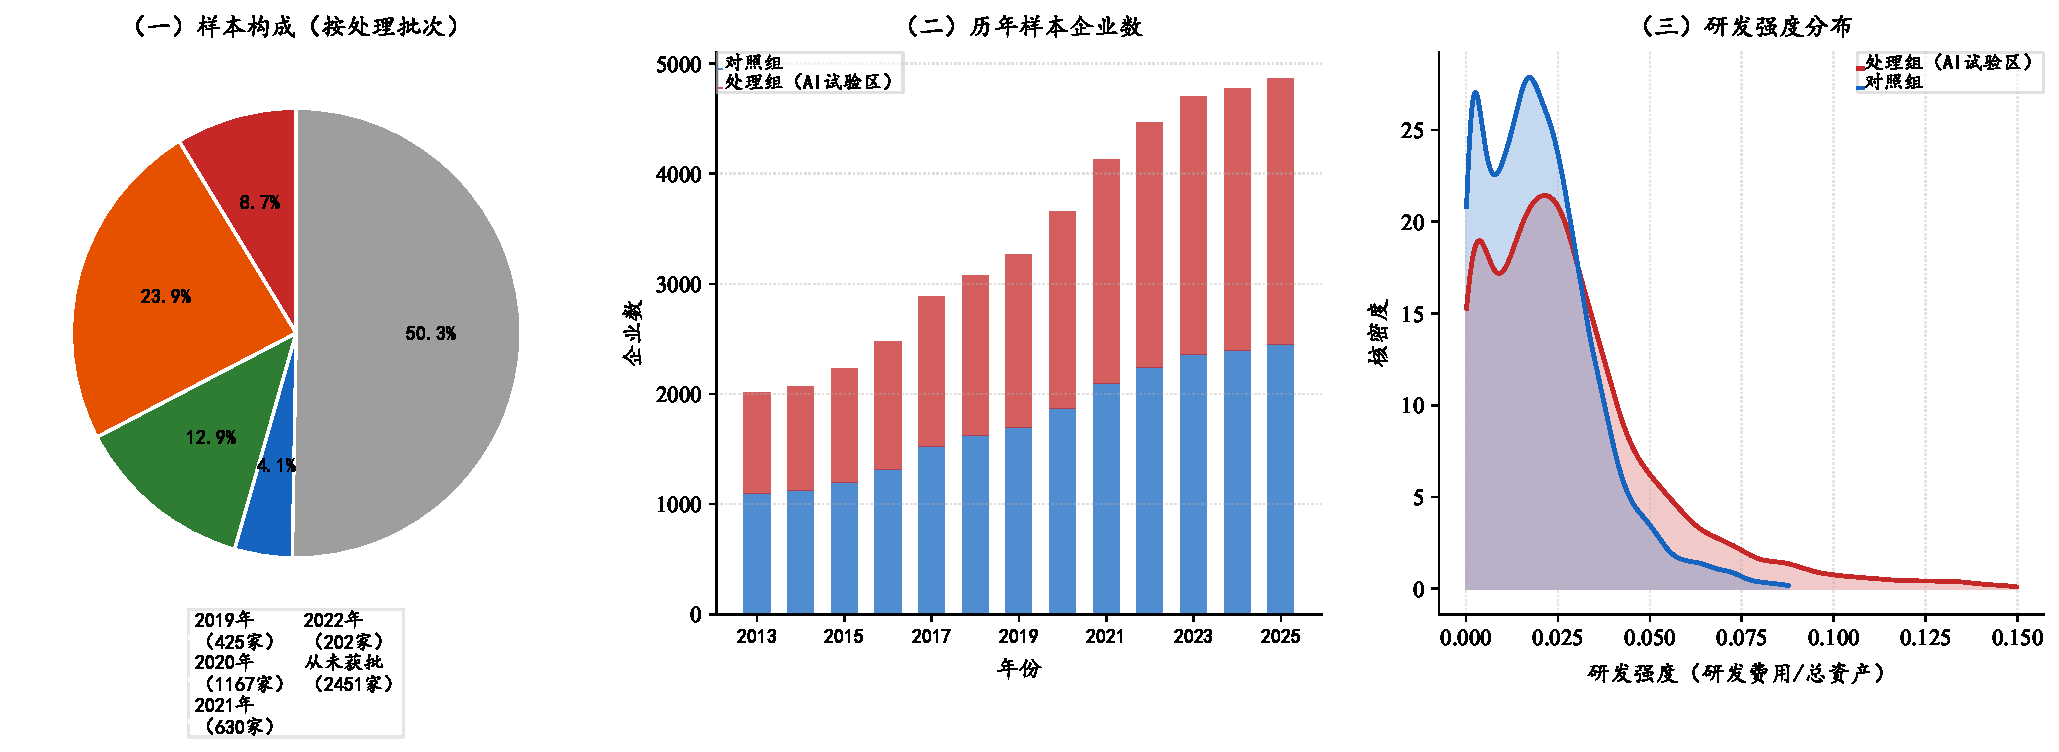
\includegraphics[width=\linewidth]{figures/fig9_样本分布_cn.pdf}
\caption{批次构成、样本量和研发分布}
\label{fig:sample}
\par\vspace{4pt}
\begin{minipage}{\linewidth}
\zihao{-5}\setlength{\baselineskip}{12pt}
注：左图百分比是占全部企业的份额。2020年批次占处理组的48.1\%，占全部企业的23.9\%。
\end{minipage}
\end{figure}

\section{估计量各自回答什么}

平均效应来自
\begin{equation}
Y_{it}=\alpha+\beta Treat_{it}+\gamma X_{it}+\mu_i+\lambda_t+\varepsilon_{it},
\label{eq:main}
\end{equation}
标准误在企业层面聚类。$\beta$混有不同批次，也混有“早获批城市对照晚获批城市”的比较。在效应接近零且各批次方向不完全相反时，它仍然是一个有用的上界：若真实的平均效应很大，这个系数很难一直停在0.0004附近。

事件研究的窗口是相对年份$-4$到$4$，省略$-1$，与图~\ref{fig:event}一致。事前系数覆盖零只说明没有检测到可分辨的事前差，事前点估计的斜率仍然要单独看\parencite{roth2023trending}。

行业式在同一套固定效应里加入$Treat_{it}\times HighAI_i$。$HighAI_i$被企业固定效应吸收。交互项是高暴露行业相对于低暴露行业的额外政策反应。低暴露行业的反应由$Treat_{it}$的主效应给出。

批次式对每个$g$只用该批次和从未处理企业。它避开了已处理对照，但每个$\delta_g$仍是该批城市与从未获批城市的双向固定效应，城市获批并不是随机的。四个系数按企业数加权等于0.00076，没有标准误，不进入推断。

\section{结果}

\subsection{平均效应有一个小的上界}

表~\ref{tab:main}第（1）列，$\hat\beta=0.0004$，聚类标准误0.0003，$t=1.38$。取标准误为$0.0004/1.38$，95\%置信区间约为$[-0.0002,\ 0.0010]$。上界0.0010相当于研发强度均值的3.9\%。预测1里“明显的平均提升”不成立；更强的说法也成立：比均值高出大约4\%以上的平均提升，与这列估计不符。第（2）列资本支出为$-0.0007$（$t=-0.78$），区间宽于研发，同样覆盖零。

\begin{table}[htbp]
\centering
\caption{平均效应}
\label{tab:main}
\begin{threeparttable}
\begin{tabular*}{\textwidth}{@{\extracolsep{\fill}}lcc}
\toprule
 & （1）研发强度 & （2）资本支出强度 \\
\midrule
Treat & 0.0004 & $-$0.0007 \\
 & (0.0003) & (0.0009) \\
95\%区间 & [$-$0.0002,\ 0.0010] & 覆盖零 \\
观测数 & 32,910 & 44,474 \\
\bottomrule
\end{tabular*}
\begin{tablenotes}
\item 注：企业和年份固定效应，标准误在企业层面聚类。研发一列的区间由系数0.0004和$t=1.38$换算，端点保留到小数第四位。
\end{tablenotes}
\end{threeparttable}
\end{table}

图~\ref{fig:event}没有给出一个迟到的显著效应。研发强度在$k=-4$为负，向$k=-1$回升；政策后前两年的点估计仍为负，第3、第4年才略高于零，每一期的95\%区间都覆盖零。这张图与表~\ref{tab:main}是同一件事：平均动态路径检测不到偏离。它不支持“三年后效应开始显现”。资本支出的事后点估计为负，区间覆盖零。图~\ref{fig:trend}的原始均值也不显示政策年有折点。

\begin{figure}[htbp]
\centering
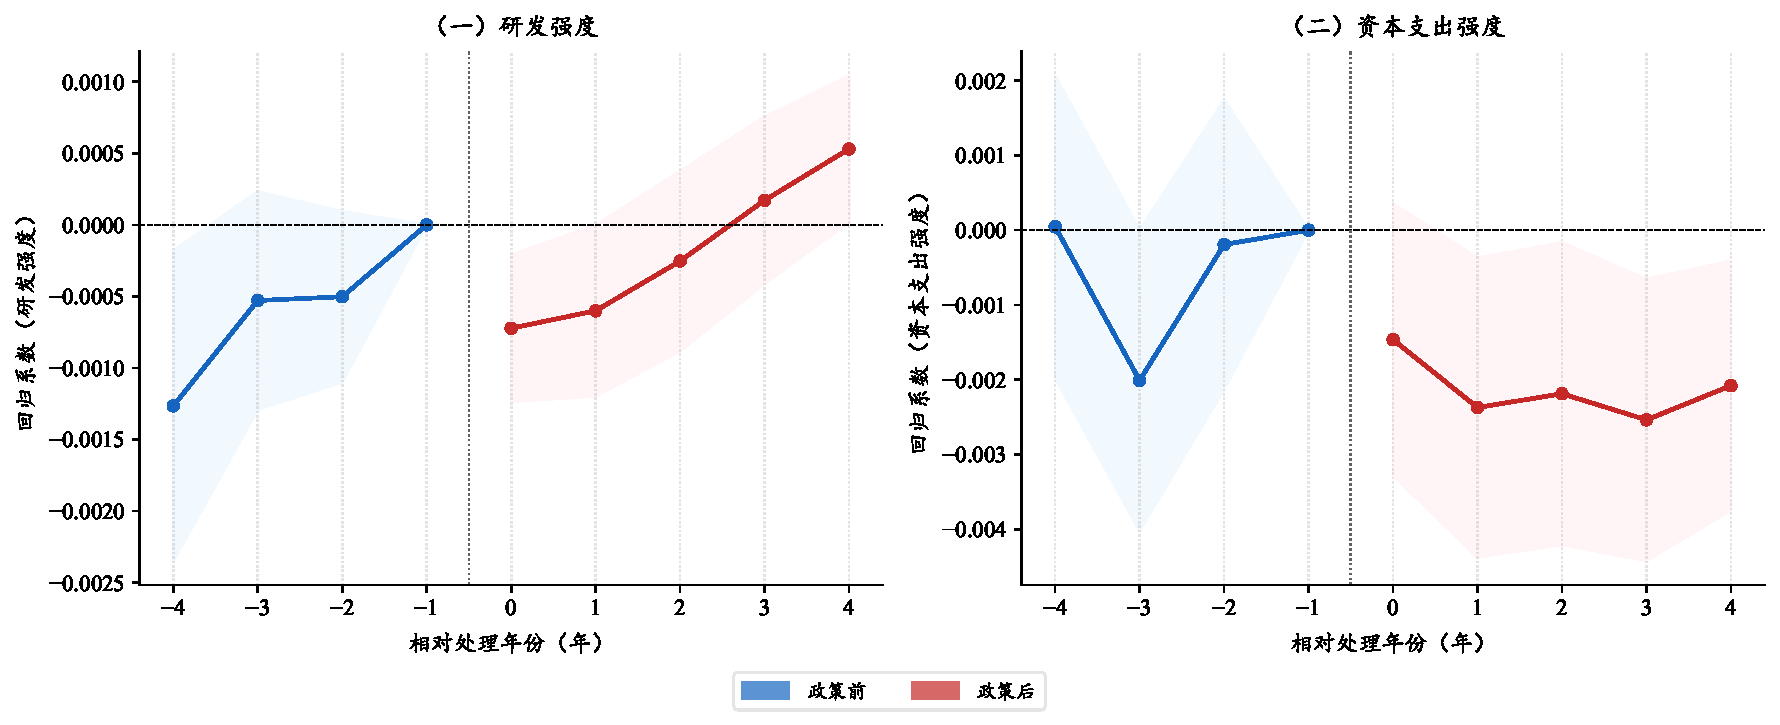
\includegraphics[width=\linewidth]{figures/fig2_事件研究_cn.pdf}
\caption{相对获批年份的系数}
\label{fig:event}
\par\vspace{4pt}
\begin{minipage}{\linewidth}
\zihao{-5}\setlength{\baselineskip}{12pt}
注：基准期$t=-1$，窗口$-4$至$4$。阴影为95\%置信区间。事前点估计斜向上升，但区间宽，不能单独拒绝平行趋势。
\end{minipage}
\end{figure}

\begin{figure}[htbp]
\centering
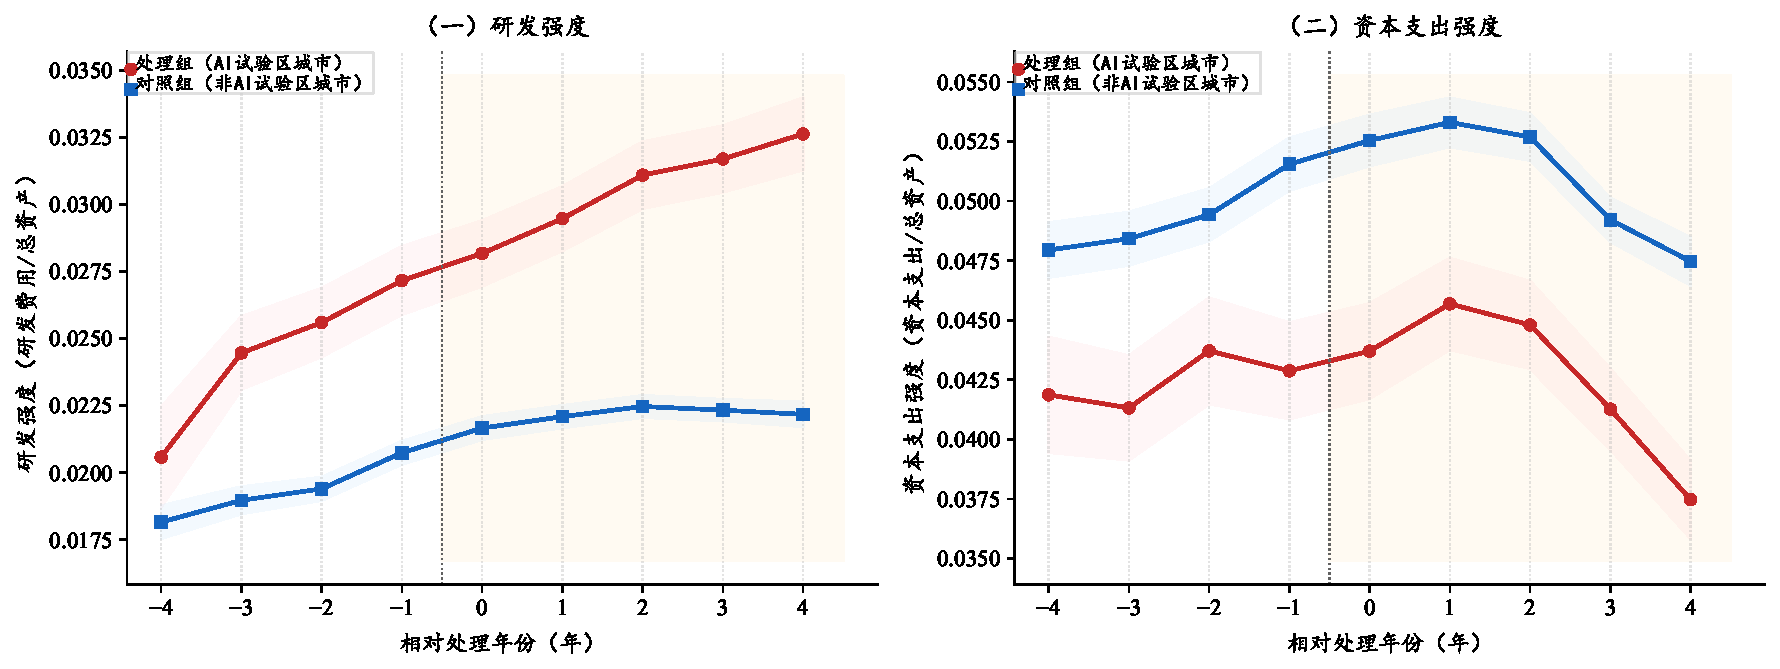
\includegraphics[width=\linewidth]{figures/fig1_趋势图_cn.pdf}
\caption{对齐后的组均值}
\label{fig:trend}
\par\vspace{4pt}
\begin{minipage}{\linewidth}
\zihao{-5}\setlength{\baselineskip}{12pt}
注：描述性叠图，不是图~\ref{fig:event}的系数。
\end{minipage}
\end{figure}

\subsection{行业对比不依赖获批年份，但事前已经在上升}

表~\ref{tab:hetero}第（1）列，交互项0.0028，$t=3.74$。低暴露行业的政策系数是$-0.0001$（$t=-0.25$）。高暴露子样本自己的系数是0.0017（$t=2.22$，5,506条观测），低暴露子样本是0.0001（$t=0.27$，27,404条）。高暴露行业只占研发样本约17\%。平均效应小，是因为多数企业所在的行业没有反应，而不是因为高暴露行业的反应也被估计成零。

这个对比不依赖“2019年的城市比2020年的城市更好”。它仍可能被行业趋势污染。图~\ref{fig:hetero_ind}左图里，高暴露组在$k=-4$大约是$-0.004$，然后一路升到基准期的零；政策当年掉回零以下，到$k=4$才略高于零，各期区间都覆盖零。低暴露组没有这条斜线。年份固定效应吸收不了“高暴露行业特有的全国趋势”。本文没有再估计带行业$\times$年份固定效应的交互项。因此交互项是全文$t$值最大的系数，不是已经去掉行业趋势的政策效应。

\begin{table}[htbp]
\centering
\caption{行业对比与两条间接渠道}
\label{tab:hetero}
\begin{threeparttable}
\begin{tabular*}{\textwidth}{@{\extracolsep{\fill}}lccc}
\toprule
 & （1）研发强度 & （2）研发强度 & （3）补贴强度 \\
\midrule
Treat & $-$0.0001 & $-$0.0001 & $-$0.0005 \\
 & [$-$0.25] &  & [$-$3.43] \\
Treat$\times$高暴露 & 0.0028 &  &  \\
 & [3.74] &  &  \\
Treat$\times$高杠杆 &  & 0.0009 &  \\
 &  & [2.10] &  \\
\bottomrule
\end{tabular*}
\begin{tablenotes}
\item 注：方括号内为$t$值。批次系数见图~\ref{fig:cohort}，不并入本表。第（3）列补贴系数取自项目结果记录。三列都有企业与年份固定效应，标准误在企业层面聚类。
\end{tablenotes}
\end{threeparttable}
\end{table}

\begin{figure}[htbp]
\centering
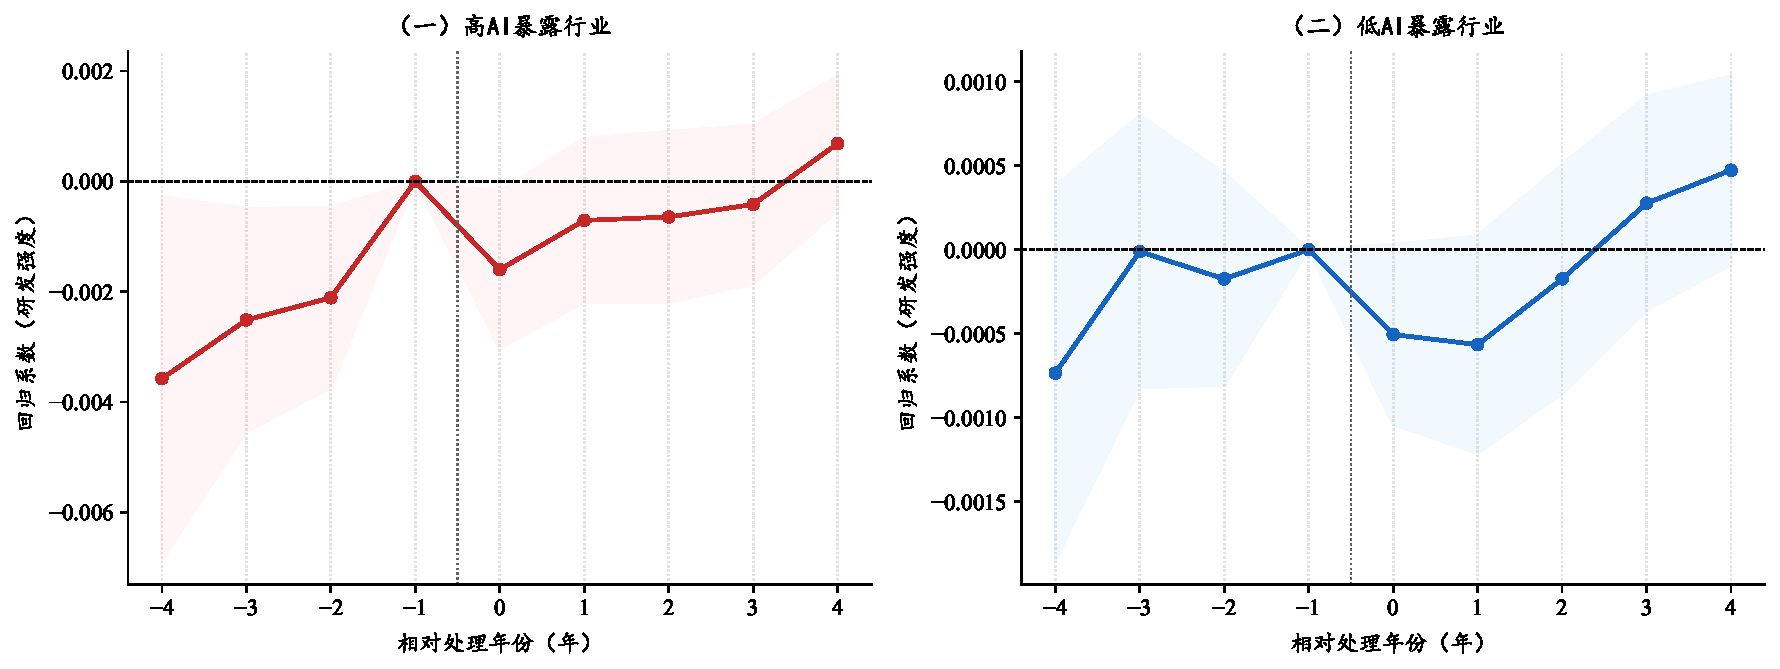
\includegraphics[width=\linewidth]{figures/fig4_异质性_cn.pdf}
\caption{高暴露行业与低暴露行业}
\label{fig:hetero_ind}
\par\vspace{4pt}
\begin{minipage}{\linewidth}
\zihao{-5}\setlength{\baselineskip}{12pt}
注：两组分开估计。高暴露组政策后的点估计更高，区间仍宽。该图没有控制行业特有的年份趋势。
\end{minipage}
\end{figure}

\subsection{批次差异是描述，不是稀释的估计}

图~\ref{fig:cohort}给出四个批次对从未处理企业的系数：2019年0.0023（$t=2.38$，$p=0.017$），2021年0.0013（$t=2.46$，$p=0.014$），2020年0.0001（$t=0.18$），2022年$-0.0001$（$t=-0.22$）。对四个批次做Bonferroni校正后，5\%的临界$p$值是0.0125。两个正的批次都略高于这个临界值。它们是未经校正时的5\%结果，不是已经过多重检验的发现。

\begin{figure}[htbp]
\centering
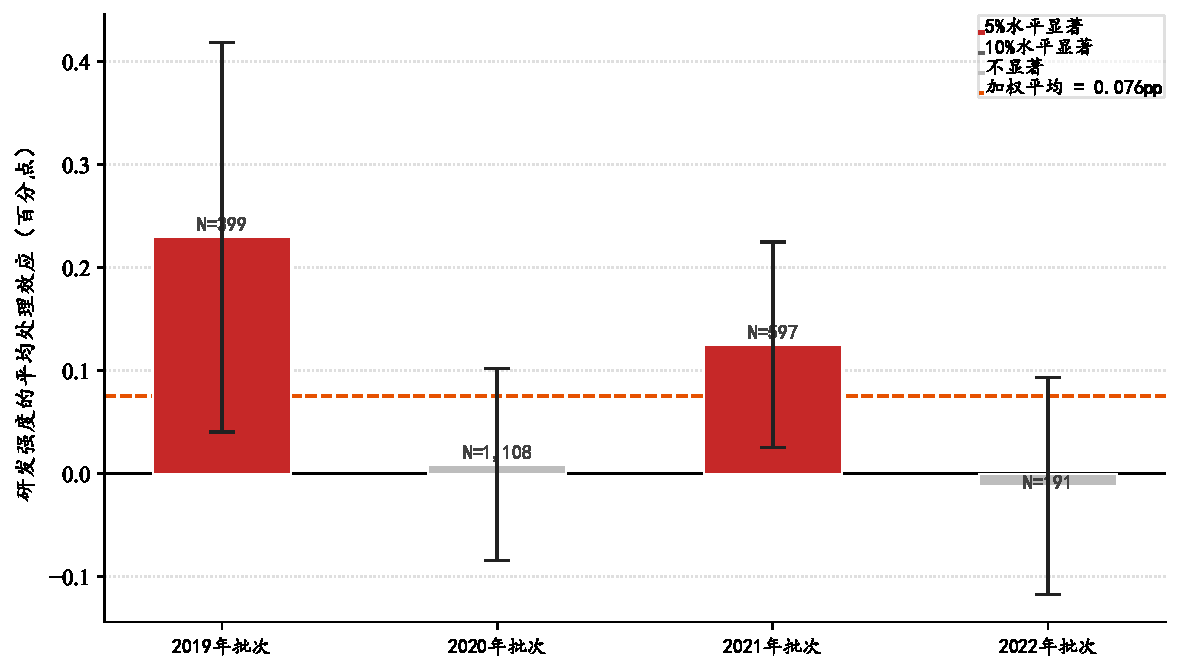
\includegraphics[width=0.85\linewidth]{figures/fig3_cohort_ATT_cn.pdf}
\caption{四个批次对从未处理企业的系数}
\label{fig:cohort}
\par\vspace{4pt}
\begin{minipage}{\linewidth}
\zihao{-5}\setlength{\baselineskip}{12pt}
注：纵轴为百分点。加权平均0.076个百分点没有标准误。2020年进入研发回归的企业是1,108家，不是全样本的1,167家。
\end{minipage}
\end{figure}

把2020年的零效应叫作稀释，需要假定这四批城市在获批时只差政策资源的厚薄。表~\ref{tab:batch}的城市名单不满足这个假定。2019年包含三座直辖市和深圳、杭州、合肥。2020年既有广州，也有郑州、济南。2020年还是疫情冲击的年份，年份固定效应只能去掉全国共同的疫情成分。2022年批次观察期止于2025年，相对年份最多到3，而图~\ref{fig:event}的研发点估计在相对年份3之前并不为正。短窗口会把一个来得晚的效应估计成零。三套解释——资源变薄、城市不同、时间不同——都预测2020或2022的系数小于2019。现有的四个数字不能在它们之间排序。

\subsection{所有制只是辅助分组}

民营企业子样本系数为0.0006（$t=1.70$，$p=0.090$），国有企业为$-0.0002$（$t=-0.40$）。图~\ref{fig:hetero_soe}与此相符，显著程度不够。同一套扩展分组里，年轻企业系数为0.0008（$t=1.77$），成熟企业接近零。方向与“预算更硬的企业反应更大”一致，也和\textcite{criscuolo2019industrial}里效应落在较小企业的结果同向，但两处都只是10\%水平的分组，本文不把它写进主要结论。

\begin{figure}[htbp]
\centering
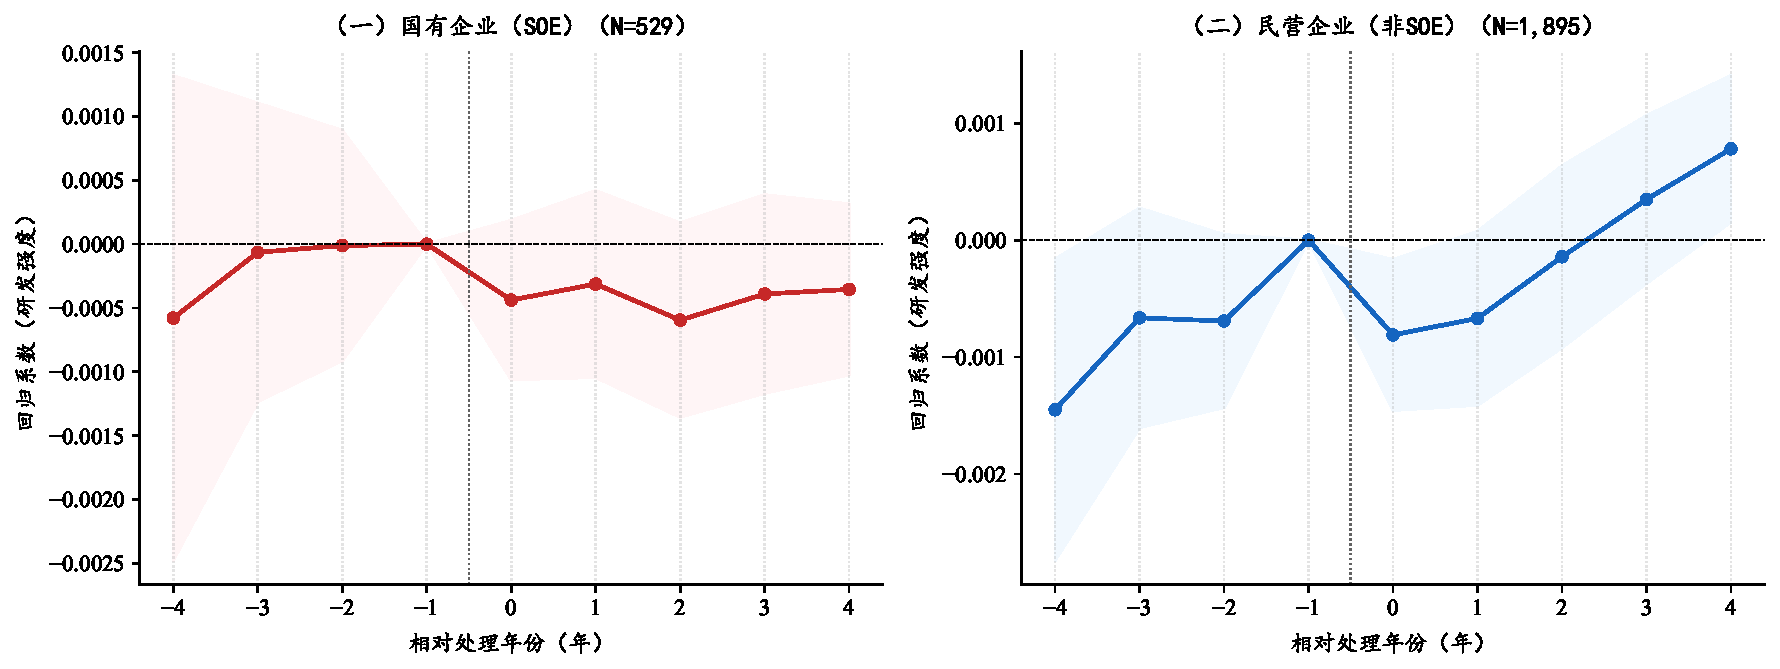
\includegraphics[width=\linewidth]{figures/fig7_所有制_cn.pdf}
\caption{国有企业与民营企业}
\label{fig:hetero_soe}
\par\vspace{4pt}
\begin{minipage}{\linewidth}
\zihao{-5}\setlength{\baselineskip}{12pt}
注：民营企业平均系数的$t$值为1.70。
\end{minipage}
\end{figure}

\section{两条渠道都还是间接的}

表~\ref{tab:hetero}第（3）列，补贴代理变量的系数是$-0.0005$（$t=-3.43$）。图~\ref{fig:mechanism}左图没有正向分叉。上市公司账上的这一定义没有因为获批而增加。\textcite{howell2017financing}的资助效应因此既没有被复制，也没有被推翻：钱若进了公共算力或未上市企业，不会出现在这个被解释变量里。税收优惠也不在分子中。

高杠杆子样本的研发系数是0.0011（$t=2.97$），低杠杆是$-0.0005$（$t=-0.99$），交互项0.0009（$t=2.10$）。这与“更缺外部资金的企业反应更大”同向，也与“借得到钱的企业杠杆更高”同向。没有利息、授信或贷款余额，交互项停在分组事实。图~\ref{fig:mechanism}右图按这个限度阅读。

\begin{figure}[htbp]
\centering

\includegraphics[width=\linewidth]{figures/fig6_机制_cn.pdf}
\caption{补贴均值与杠杆分组系数}
\label{fig:mechanism}
\par\vspace{4pt}
\begin{minipage}{\linewidth}
\zihao{-5}\setlength{\baselineskip}{12pt}
注：右图不是信贷价格。高杠杆按样本中位数划分。
\end{minipage}
\end{figure}

\section{平均效应的敏感性}

表~\ref{tab:robust}把平均系数放在三种替代设定里。省份$\times$年份固定效应下为0.0008（$t=1.71$），2018年倾向得分匹配后为0.0006（$t=1.75$，18,429条；匹配变量为规模、杠杆、资产收益率和年龄，最近邻，卡尺0.05），去掉北京、上海、天津、重庆后为0.0006（$t=1.67$）。三列都在10\%的边上，没有一列达到5\%。点估计没有离开基准的数量级。平均效应对设定是稳定地小，不是稳定地显著。

\begin{table}[htbp]
\centering
\caption{平均系数的三种替代设定}
\label{tab:robust}
\begin{threeparttable}
\begin{tabular*}{\textwidth}{@{\extracolsep{\fill}}lccc}
\toprule
 & 省份$\times$年份 & 匹配样本 & 去掉直辖市 \\
\midrule
Treat & 0.0008 & 0.0006 & 0.0006 \\
$t$值 & 1.71 & 1.75 & 1.67 \\
观测数 & 32,907 & 18,429 & 26,583 \\
\bottomrule
\end{tabular*}
\begin{tablenotes}
\item 注：被解释变量为研发强度。匹配在处理前的2018年进行。去掉直辖市并不等于重估2019年批次，深圳仍留在样本里。
\end{tablenotes}
\end{threeparttable}
\end{table}

\begin{figure}[htbp]
\centering
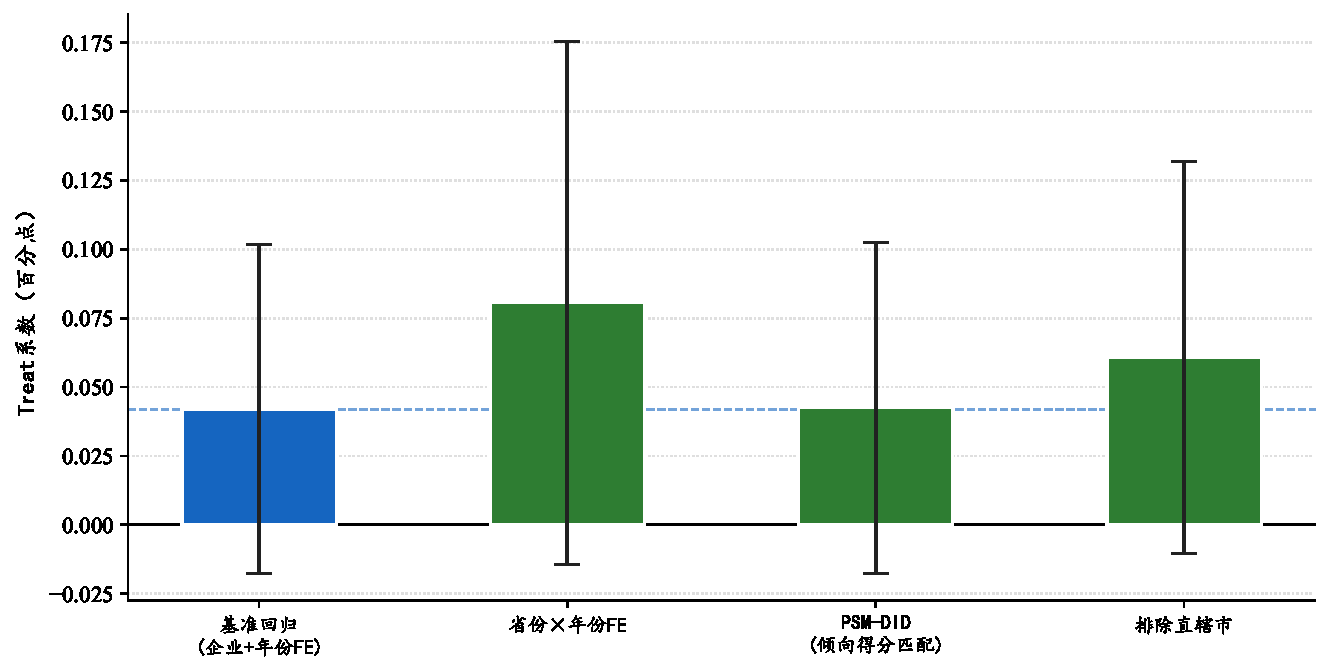
\includegraphics[width=0.82\linewidth]{figures/fig8_稳健性_cn.pdf}
\caption{替代设定下的平均系数}
\label{fig:robust_coef}
\par\vspace{4pt}
\begin{minipage}{\linewidth}
\zihao{-5}\setlength{\baselineskip}{12pt}
注：95\%置信区间。读这张图的方式是区间的位置和宽度，不是星号。
\end{minipage}
\end{figure}

图~\ref{fig:placebo}不能承担安慰剂的主要工作。它随机保留一部分公司的原有$Treat$、把其余公司置零，重复300次，真实系数高于55.7\%的抽取值。从未处理的公司不会因此获得一条伪处理路径。把获批年份在公司之间打乱的500次练习更接近随机化推断，真实系数高于其中55.4\%。平均效应处在噪声的中部。这个结果强化的是“平均效应检测不到”，不是“隐藏的正效应很稳健”。

\begin{figure}[htbp]
\centering
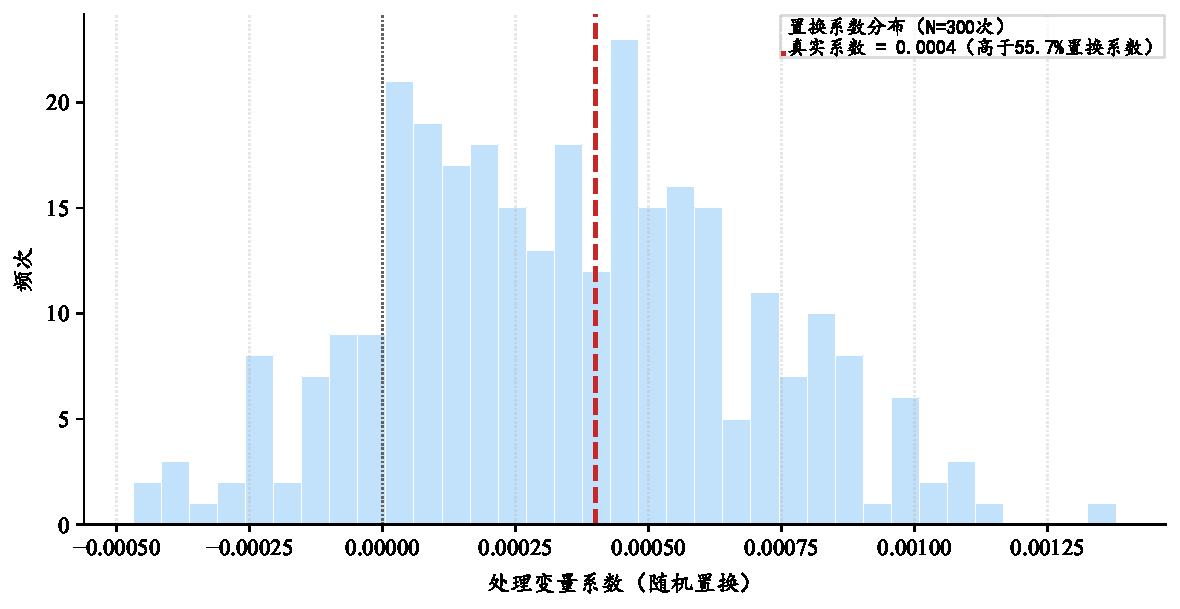
\includegraphics[width=0.78\linewidth]{figures/fig5_安慰剂_cn.pdf}
\caption{图内的300次抽取}
\label{fig:placebo}
\par\vspace{4pt}
\begin{minipage}{\linewidth}
\zihao{-5}\setlength{\baselineskip}{12pt}
注：正式的时点置换是另一套500次练习，百分位数为55.4。两套结果都在分布中部。
\end{minipage}
\end{figure}

还没有做、而且会改变解释的检验包括：行业$\times$年份固定效应下的交互项，去掉直辖市后的分批次系数，以及研发是否披露对获批的回归。年轻企业那一项10\%水平的系数也属于扩展分组，不是预先写定的检验。

\section{结\quad 论}

试验区没有把上市公司的平均研发强度提高一个在经济上值得写出的幅度。95\%置信区间的上界大约是均值的4\%。资本支出没有可检测的变化。高人工智能暴露行业相对于低暴露行业有0.28个百分点的额外反应，$t$值是全文最大的，但高暴露组在政策前已经向零回升，这个对比还没有去掉行业自己的年份趋势。2019年和2021年批次的正系数、2020年批次的零系数是清楚的描述；稀释、城市选择、疫情和短窗口都能产生这张表，本文没有在它们之间做出识别。

因此政策句子也只有两句可以写。第一，用全体上市公司的平均研发去评价这项城市政策，会得到一个很紧的零，这个零主要反映低暴露行业。评价应事先限定在使用算力和数据的行业。第二，在没有贷款价格、也没有把批次和城市基础分开之前，不宜从2020年的零效应推出“试点应当保持小规模”，也不宜推出“试点应当继续扩大”。两种建议都比这四批城市所能识别的内容多走了一步。

专利、研发人员地点和未上市企业都不在样本里。注册地不等于研发发生地。试验区不是抽签产生的。这些边界和置信区间是一起读的。

\printbibliography[title={参考文献}]

\enmaketitle
\end{document}
